% Assignment 3 report - Load Balancing and Observability (Paws & Cart behind Envoy)
% Compile: pdflatex assignment3-report.tex   (run twice so figure numbers are filled in)
% Needs the folder figures/ next to this file (Grafana, Prometheus and Kibana screenshots).
\documentclass[10pt,a4paper]{article}
\usepackage[margin=2cm]{geometry}
\usepackage[T1]{fontenc}
\usepackage{lmodern}
\usepackage{microtype}
\usepackage{graphicx}
\usepackage{booktabs}
\usepackage{tabularx}
\usepackage{array}
\usepackage{xcolor}
\usepackage{float}
\usepackage{tikz}
\usetikzlibrary{positioning,arrows.meta,calc}
\usepackage[font=small,labelfont=bf]{caption}
\usepackage{subcaption}
\usepackage{enumitem}
\usepackage[hidelinks]{hyperref}
\setlist{nosep,leftmargin=1.4em}
\setlength{\parskip}{4pt}
\setlength{\parindent}{0pt}
\setlength{\emergencystretch}{1.5em}
\newcolumntype{Y}{>{\raggedright\arraybackslash}X}
\newcolumntype{L}[1]{>{\raggedright\arraybackslash}p{#1}}
\newcolumntype{C}[1]{>{\centering\arraybackslash}p{#1}}
% inline code that may break after an underscore
\newcommand{\codeus}{\textunderscore\allowbreak}
\newcommand{\code}[1]{{\small\ttfamily\let\_\codeus #1}}
% one Grafana/Kibana screenshot inside a figure
\newcommand{\shot}[3][0.49\textwidth]{\begin{subfigure}[t]{#1}\centering
  \includegraphics[width=\linewidth]{figures/#2}\caption{#3}\end{subfigure}}
% prediction / observation / explanation labels for Part D
\newcommand{\pred}{\textbf{Prediction.} }
\newcommand{\obs}{\textbf{Observation.} }
\newcommand{\expl}{\textbf{Explanation.} }

\title{\vspace{-1.2cm}Assignment 3: Load Balancing and Observability\\[2pt]
\large Paws \& Cart pet shop behind Envoy}
\author{Zainab Bhutto \\ \small Enterprise Software Development, Fall 2026}
\date{\small November 2026 \quad Code: \href{https://github.com/zainabsbhutto02/petstore-observability}{github.com/zainabsbhutto02/petstore-observability}}

\begin{document}
\maketitle
\vspace{-0.5cm}

\section*{Summary}

I ran three copies (replicas A, B and C) of my Assignment 2 shop behind an \textbf{Envoy} proxy. I then measured
how Envoy shares HTTP requests and gRPC calls between them, using the observability stack from Assignments 1 and 2:
Prometheus and Grafana for metrics, and Filebeat, Elasticsearch and Kibana for logs. Every test used the
\textbf{same workload}: a fixed-rate client sending \textbf{20 requests per second for 90 seconds} (1800 requests),
without waiting for answers and without retries. HTTP tests call \code{GET /products}, gRPC tests call
\code{ListProducts}. Both are read-only, so they do not use up stock. All charts are screenshots of my Grafana
dashboard, taken for each test's own time window. Grafana shows local time (UTC+5).

\section{Part A: Replicas, routing and shared state}

\subsection{Architecture}

\begin{figure}[H]
\centering
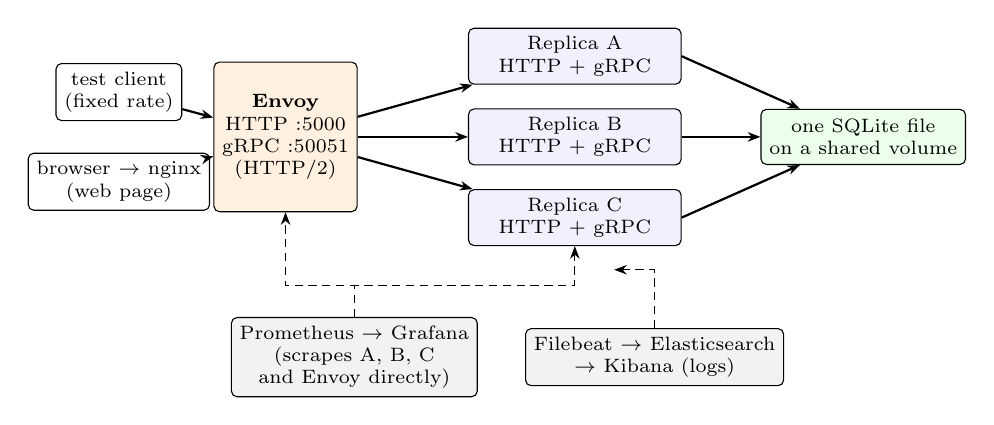
\begin{tikzpicture}[font=\scriptsize, node distance=4mm and 9mm,
  box/.style={draw, rounded corners=2pt, align=center, inner sep=3pt, minimum height=7mm},
  rep/.style={box, fill=blue!6, minimum width=27mm},
  obs/.style={box, fill=gray!10},
  arr/.style={-{Stealth[length=1.6mm]}, thick},
  feed/.style={-{Stealth[length=1.6mm]}, densely dashed}]
\node[box] (lg) {test client\\(fixed rate)};
\node[box, below=of lg] (web) {browser $\to$ nginx\\(web page)};
\node[box, fill=orange!12, right=12mm of $(lg)!0.5!(web)$, minimum height=19mm] (envoy)
  {\textbf{Envoy}\\HTTP :5000\\gRPC :50051\\(HTTP/2)};
\node[rep, right=14mm of envoy] (b) {Replica B\\HTTP + gRPC};
\node[rep, above=3mm of b] (a) {Replica A\\HTTP + gRPC};
\node[rep, below=3mm of b] (c) {Replica C\\HTTP + gRPC};
\node[box, fill=green!8, right=10mm of b] (db) {one SQLite file\\on a shared volume};
\node[obs, below=9mm of c, xshift=-28mm] (prom) {Prometheus $\to$ Grafana\\(scrapes A, B, C\\and Envoy directly)};
\node[obs, right=6mm of prom] (elk) {Filebeat $\to$ Elasticsearch\\$\to$ Kibana (logs)};
\draw[arr] (lg) -- (envoy);
\draw[arr] (web) -- (envoy);
\draw[arr] (envoy) -- (a); \draw[arr] (envoy) -- (b); \draw[arr] (envoy) -- (c);
\draw[arr] (a.east) -- (db); \draw[arr] (b) -- (db); \draw[arr] (c.east) -- (db);
\draw[feed] (prom.north) -- ++(0,4mm) -| (envoy.south);
\draw[feed] (prom.north) -- ++(0,4mm) -| (c.south);
\draw[feed] (elk.north) |- ($(c.south)+(5mm,-3mm)$);
\end{tikzpicture}
\caption{Architecture. Solid arrows carry requests. Dashed arrows are monitoring: Prometheus scrapes each replica and
Envoy directly (not through the balanced route), and Filebeat collects the logs of all containers.}
\label{fig:arch}
\end{figure}

\begin{itemize}
\item \textbf{Three replicas with Docker Compose scaling.} The shop is one Compose service with
\code{deploy.replicas: 3}. Each replica runs the REST API and the gRPC service together, so A, B and C offer the same
HTTP endpoints and gRPC methods.
\item \textbf{Envoy is the only way in.} It listens on port 5000 for HTTP and 50051 for gRPC. In Part A both routes
send everything to \textbf{A only}. B and C keep running but are not Envoy destinations yet.
\item \textbf{Replica identifier.} Each replica knows its letter (A, B or C) and adds it to every log line
(\code{"replica":"B"}) and to every response (header \code{X-Replica}). In Prometheus each replica is a separate target
with the label \code{replica}.
\item \textbf{Request correlation.} Envoy gives every request an \code{X-Request-ID} (or keeps the client's) and
passes it on, for gRPC too. Envoy and the replica both log this ID, so one search finds both events
(Section~\ref{sec:logs}).
\end{itemize}

\subsection{Shared or separate state}

\begin{table}[H]
\centering\small
\begin{tabularx}{\textwidth}{@{}l l Y@{}}
\toprule
State & Shared or separate? & What happens when requests are spread over A, B and C \\
\midrule
Data (products, stock, orders) & \textbf{Shared}: one SQLite file on a shared volume &
Nothing goes wrong. Every replica reads and writes the same rows, and writes are done one at a time inside a
transaction, so stock stays correct. \\
Idempotency records & \textbf{Shared}: a table in the same SQLite file &
Nothing goes wrong. A retry with the same \code{Idempotency-Key} returns the original order on any replica, so
duplicate orders are still prevented. \\
Rate-limit counters & \textbf{Separate}: kept in each replica's memory &
The limit breaks. Each replica allows 10 orders per minute per client, so with three replicas a client gets about
\textbf{30 per minute instead of 10}. A client blocked on A can still order through B, and the
\code{Retry-After} time depends on which replica answered. Fix (not implemented): keep the counters in a shared
store such as Redis. \\
\bottomrule
\end{tabularx}
\caption{Which state is shared by all replicas and which is kept separately in each replica.}
\label{tab:state}
\end{table}

\subsection{Envoy, health-check and metric settings}

\begin{itemize}
\item \textbf{Envoy listeners.} The HTTP listener is plain HTTP/1.1. The gRPC listener uses \textbf{HTTP/2}, so
Envoy sees every gRPC call separately. There are no retries, and the timeout is 5\,s. For a comparison in Part C,
a third listener sends gRPC through a plain \textbf{TCP proxy}. Each experiment has its own small Envoy config file,
which differs from the round-robin file only in its balancing settings.
\item \textbf{Active health checks} (used in D.3). HTTP checks call \code{GET /health}, and gRPC checks use the
standard gRPC health service. Table~\ref{tab:hc} gives the settings.
\end{itemize}

\begin{table}[H]
\centering\small
\begin{tabular}{@{}l l l@{}}
\toprule
Setting & Value & Meaning \\
\midrule
Interval & 2\,s & each replica is checked every 2 seconds \\
Timeout & 1\,s & a check that takes longer than 1 second fails \\
Unhealthy threshold & 2 & 2 failed checks in a row $\to$ replica removed \\
Healthy threshold & 2 & 2 passed checks in a row $\to$ replica added back \\
\bottomrule
\end{tabular}
\caption{Active health-check settings (the same for HTTP and gRPC).}
\label{tab:hc}
\end{table}

\textbf{Metrics and queries.} Prometheus scrapes A, B, C and Envoy \textbf{directly}, every 5\,s, never through
Envoy (Figure~\ref{fig:targets}). The Grafana dashboard \emph{``Paws \& Cart - A3 Load Balancing (per replica)''} has
one row for HTTP and one for gRPC, with these panels per replica:

\begin{table}[H]
\centering\small
\begin{tabularx}{\textwidth}{@{}l Y l@{}}
\toprule
Panel & Main PromQL query (HTTP; the gRPC panels use the gRPC metrics) & Time window \\
\midrule
Request rate & \code{sum by (replica) (rate(petstore\_http\_request\_duration\_seconds\_count[1m]))} & 1 minute \\
Share of total & replica rate $\div$ total rate, with a dashed line at 33\,\% & 1 minute \\
Share over the time range & \code{increase(...[\$\_\_range])} per replica $\div$ total & whole chosen range \\
Active requests & \code{petstore\_http\_requests\_in\_flight}, \code{grpc\_server\_in\_flight\_requests} & 5\,s samples \\
p50 / p95 time & \code{histogram\_quantile(0.95, sum by (replica, le) (rate(..\_bucket[1m])))} & 1 minute \\
Errors by status & non-2xx HTTP codes or non-OK gRPC codes, plus errors created by Envoy & 1 minute \\
\bottomrule
\end{tabularx}
\caption{Dashboard panels and their queries.}
\label{tab:queries}
\end{table}

Metric labels only take a few fixed values (replica, route, status code, gRPC method). Request IDs are never used as
labels; they appear only in logs.

\begin{figure}[H]
\centering
\shot[0.8\textwidth]{prom-targets-app.jpg}{Targets A, B and C (job \code{petstore-app})}
\\[4pt]
\shot[0.8\textwidth]{prom-targets-envoy.jpg}{Target Envoy (job \code{envoy})}
\caption{Prometheus scrapes each replica by its own container name, with the label \code{replica}, and Envoy's
metrics page. All four targets are UP.}
\label{fig:targets}
\end{figure}

\section{Part B: Baseline, Envoy sends everything to A}

\textbf{Observed.} A handled \textbf{all} requests and calls. B and C were running and healthy but idle, as expected
(Figure~\ref{fig:baseline}). The client got 1800 out of 1800 successful answers on both interfaces. Client p95 was
26.3\,ms for HTTP and 10.0\,ms for gRPC.

\begin{figure}[H]
\centering
\shot{b-http-rate.jpg}{HTTP request rate per replica}
\hfill
\shot{b-http-share.jpg}{HTTP share over the run: A 100\,\%}
\\[4pt]
\shot{b-grpc-rate.jpg}{gRPC call rate per replica}
\hfill
\shot{b-grpc-share.jpg}{gRPC share over the run: A 100\,\%}
\caption{Part B baseline (HTTP run, then gRPC run). Only A has traffic; B and C stay at 0.}
\label{fig:baseline}
\end{figure}

\subsection{Logs: the Envoy event together with the replica event}
\label{sec:logs}

Envoy writes a JSON access log line for every request. It contains the request ID, the chosen replica
(\code{replica}) and its address (\code{upstream\_host}). Filebeat sends these lines to Elasticsearch together with
the replicas' own JSON logs. In Kibana, \textbf{one search for a request ID returns both events}
(Figure~\ref{fig:kibana}). These are the two proxy and backend log examples. They are taken from the Part C runs, so
that they show replicas other than A:

\begin{itemize}
\item \textbf{HTTP} (\code{request\_id:"rr-equal-http-ecd47c-000100"}): Envoy logged \code{listener=http},
\code{replica=B}, \code{upstream\_host=172.18.0.10:5000} and status 200. Replica B logged the same request ID for
\code{/products}, status 200.
\item \textbf{gRPC} (\code{request\_id:"rr-equal-grpc-8d3864-000100"}): Envoy logged \code{listener=grpc},
\code{replica=C}, \code{upstream\_host=172.18.0.2:50051} and \code{grpc\_status=OK}. Replica C logged the same ID for
\code{ListProducts}, code OK.
\end{itemize}

\begin{figure}[H]
\centering
\shot[\textwidth]{kibana-http.jpg}{HTTP: one search returns the replica event (\code{pet-store}, B) and the Envoy event (B, 172.18.0.10:5000).}
\\[4pt]
\shot[\textwidth]{kibana-grpc.jpg}{gRPC: one search returns the replica event (\code{pet-store-grpc}, C) and the Envoy event (C, 172.18.0.2:50051).}
\caption{Kibana Discover: the proxy event and the backend event share the same request ID.}
\label{fig:kibana}
\end{figure}

\section{Part C: Equal round robin}

B and C were added to Envoy's destinations with equal weights. The same workload was run again.

\textbf{Observed.} Each replica received about one third of the traffic, on both interfaces
(Figure~\ref{fig:rr}). Grafana shows 33.3 / 33.3 / 33.4\,\% for HTTP and 32.6 / 33.7 / 33.7\,\% for gRPC. Envoy's
access log gives the exact counts: \textbf{600 / 600 / 600} for both. The small Grafana difference comes from how
Prometheus estimates a count at the edges of a time window. All requests succeeded. Client p95 was 8.8\,ms for HTTP
and 8.2\,ms for gRPC.

\textbf{Difference from the A-only baseline.} The shares changed from 100/0/0 to about 33/33/33. Client p95 is lower
than in the baseline (26.3 $\to$ 8.8\,ms for HTTP), but that is mostly \emph{not} extra capacity. On the server, p95
was below 5\,ms in both runs, so A alone was never overloaded. The higher baseline value came from a short Docker
Desktop pause during that run, which delayed 15 client sends.

\textbf{gRPC: per call, not per connection.} A gRPC client opens \textbf{one} connection and sends every call
through it. Through Envoy's HTTP/2 listener that single connection was split 600/600/600, because Envoy routes each
call. Through the TCP-proxy listener, Envoy only sees the connection, so it chose a replica once and
\textbf{all 1800 calls went to A} (Figure~\ref{fig:rr}e).

\begin{figure}[H]
\centering
\shot{c-http-sharets.jpg}{HTTP share over time: all three on the 33\,\% line}
\hfill
\shot{c-http-share.jpg}{HTTP share over the run}
\\[4pt]
\shot{c-grpc-sharets.jpg}{gRPC share over time (HTTP/2 listener)}
\hfill
\shot{c-grpc-share.jpg}{gRPC share over the run}
\\[4pt]
\shot{c-tcp-share.jpg}{gRPC through a plain TCP proxy: one connection, so 100\,\% on A}
\caption{Part C, equal round robin. The share bars (b, d) are the values to compare with 33\,\%. The ``Mean'' values in
the legends of (a) and (c) include the time before each run started, so they are not the run's shares. The first point
of (a) shows A at 100\,\% because B and C had no earlier HTTP data, and Prometheus needs two samples before it can
compute a rate.}
\label{fig:rr}
\end{figure}

\section{Part D: Experiments}

Every experiment started from the healthy round-robin setup of Part C. Each used the same workload and was undone
afterwards. Client retries and circuit breakers were off.

\subsection{D.1 Weighted round robin (A:B:C = 2:1:1)}

\pred A should get 50\,\% and B and C 25\,\% each. Latency and active requests should hardly change, because even
10 requests per second is light work for one replica.

\obs The shares were 49.8 / 25.1 / 25.1\,\% for HTTP and 50.8 / 24.5 / 24.6\,\% for gRPC in Grafana
(Figure~\ref{fig:d1}). Envoy's log counted 899 / 451 / 450 and 900 / 450 / 450. Server p95 stayed below 5\,ms on all
three replicas (the chart shows 4.8\,ms because 5\,ms is the smallest histogram bucket). Active requests stayed near 0. Client p95 went from 8.8 to 10.2\,ms (HTTP) and from 8.2 to 8.7\,ms
(gRPC). There were no errors.

\expl Envoy follows the weights very closely. A weight only \emph{moves} traffic and does not add capacity. A could
take twice the traffic here only because it had plenty of spare capacity. If A were the slowest replica, giving it
weight 2 would make things worse, so weights should match each replica's real capacity.

\begin{figure}[H]
\centering
\shot{d1-http-share.jpg}{HTTP share}
\hfill
\shot{d1-grpc-share.jpg}{gRPC share}
\\[4pt]
\shot{d1-http-p95.jpg}{HTTP p50 / p95: about the same on A, B and C}
\caption{D.1 weighted round robin 2:1:1. Shares close to 50/25/25; response time unchanged.}
\label{fig:d1}
\end{figure}

\subsection{D.2 Least request with a slow replica}

B was made slow on purpose: it waits 200\,ms before answering each \code{/products} request or \code{ListProducts}
call. Its health endpoint was not slowed down, so B still passed health checks. The same workload ran twice: once
with round robin and once with \textbf{least request}. With equal weights, least request picks two replicas at random
and sends the request to the one with fewer requests in progress.

\pred With round robin, B keeps 33\,\% of the traffic, so a third of all requests take about 200\,ms and client p95
is about 200\,ms. With least request, B is usually busy, so it gets fewer new requests. p95 only improves if B's
share drops below 5\,\%.

\obs (Figure~\ref{fig:d2})
\begin{itemize}
\item \textbf{Round robin:} B kept 33.4\,\% (HTTP) and 33.3\,\% (gRPC). B had 1--3 requests in progress while A and C
had 0. B's p95 was about 243\,ms, and client p95 was 209\,ms (HTTP) and 208\,ms (gRPC).
\item \textbf{Least request:} B's share \textbf{fell to 19.7\,\% (HTTP) and 17.9\,\% (gRPC)}, and A and C took the
rest. B served 355 instead of 601 HTTP requests and 322 instead of 600 gRPC calls. For gRPC, B's average number of
active calls halved (1.3 $\to$ 0.7). For HTTP the 5-second samples stayed about the same (1.4), because a short Docker
pause in that run held back 16 sends and then released them together. Client p95 was still 212\,ms (HTTP) and
208\,ms (gRPC), and p50 hardly changed (8.3 $\to$ 8.2\,ms HTTP, 7.5 $\to$ 7.1\,ms gRPC).
\item There were no errors in any run.
\end{itemize}

\expl Least request sends new work away from a replica that is still busy. Round robin ignores how busy a replica is.
At 20 requests per second, A and C are almost never busy, so B only gets a request when it happens to be idle too.
That is why its share fell to about a fifth, and the number of slow answers dropped by 41\,\% (HTTP) and 46\,\%
(gRPC). However, p95 looks at the slowest 5\,\% of requests. B still served about 18--20\,\% of all requests, so the
slowest 5\,\% were still B's 200\,ms answers and p95 did not move. p50 did not move either, because most requests were
fast in both runs. With more load, or a stronger least-request setting, B's share would fall further.

\begin{figure}[H]
\centering
\shot{d2rr-http-share.jpg}{Round robin: HTTP share (B 33\,\%)}
\hfill
\shot{d2lr-http-share.jpg}{Least request: HTTP share (B 19.7\,\%)}
\\[4pt]
\shot{d2rr-http-active.jpg}{Round robin: active HTTP requests (B up to 3)}
\hfill
\shot{d2lr-http-active.jpg}{Least request: active HTTP requests (B only; chart points every 15\,s)}
\\[4pt]
\shot{d2rr-http-p95.jpg}{Round robin: p50 / p95 (B about 243\,ms)}
\hfill
\shot{d2lr-http-p95.jpg}{Least request: p50 / p95 (B still slow)}
\\[4pt]
\shot{d2rr-grpc-share.jpg}{Round robin: gRPC share (B 33.5\,\%)}
\hfill
\shot{d2lr-grpc-share.jpg}{Least request: gRPC share (B 17.9\,\%)}
\caption{D.2, B slowed by 200\,ms. Left: round robin. Right: least request with the same delay and workload. B's
measured 243\,ms is slightly above the real 210\,ms because of the histogram bucket size.}
\label{fig:d2}
\end{figure}

\subsection{D.3 Failure and recovery}

Round robin, no delay, with the active health checks from Table~\ref{tab:hc}. During each 90-second run, B was
stopped (\code{docker stop}) at +20\,s and started again (\code{docker start}) at +50\,s. A script recorded the
exact times from Envoy.

\pred Envoy needs 2 failed checks, 2\,s apart, to remove B. That takes about 2 to 5\,s after B stops. Until then about
one third of the requests fail. After B starts again, it needs 2 passed checks (about 2 to 4\,s) before it gets
traffic again.

\obs (Figure~\ref{fig:d3})
\begin{itemize}
\item \textbf{Removal:} B was marked unhealthy \textbf{4.2\,s} after the stop for HTTP and \textbf{6.7\,s} for gRPC.
For gRPC, the stop signal reached B 1.5\,s late, and B finished its open calls for up to 2\,s before closing.
\item \textbf{Errors:} the client saw \textbf{24 errors} for HTTP (1.33\,\%, all \code{503}) and \textbf{32 errors}
for gRPC (1.78\,\%, all \code{UNAVAILABLE}). All of them happened \emph{before} B was removed. After that, A and C
took about 10 requests per second each, with no errors.
\item \textbf{Recovery:} B needed 7.6\,s (HTTP run) and 5.0\,s (gRPC run) just to start. Envoy then marked it healthy
3.3\,s later in the HTTP run, which is 2 passed checks. In the gRPC run it took 0.7\,s, because Envoy needs only one
passed check for a replica it has just re-added. No requests failed during recovery.
\item Envoy's healthy-endpoint count went 3 $\to$ 2 $\to$ 3 in both runs. About 1--3\,s after the health check removed
B, Docker's DNS also stopped listing B, so Envoy's \emph{total} endpoint count dropped to 2 as well. The health check
was first in both runs.
\end{itemize}

\expl How long removal takes is set by the health-check settings: about \emph{interval $\times$ unhealthy threshold},
plus the timeout. The number of errors is that time multiplied by B's share of the traffic: about 6.7 requests per
second for 4--5\,s gives 24--32 errors. Recovery is B's start-up time plus about 2 checks. A shorter interval, or one
retry for read-only requests, would reduce these errors; retries were turned off on purpose for this test.

\begin{figure}[H]
\centering
\shot{d3-http-rate.jpg}{HTTP request rate: B drops out, A and C take over}
\hfill
\shot{d3-http-errors.jpg}{HTTP errors: Envoy returned 503 until B was removed}
\\[4pt]
\shot{d3-grpc-rate.jpg}{gRPC call rate during the gRPC run}
\hfill
\shot{d3-grpc-errors.jpg}{gRPC errors: calls that failed in Envoy before reaching a replica}
\\[4pt]
\shot{d3-envoy-healthy.jpg}{Envoy endpoints: 3 $\to$ 2 $\to$ 3 in each run. The light line (healthy) drops first; the
dark line (total) follows when DNS drops B. The gRPC lines lie under the HTTP lines.}
\caption{D.3: B stopped at +20\,s and restarted at +50\,s (HTTP run first, then the gRPC run). Values use a 1-minute
window, so short events look wider than they were. The exact times are in the text.}
\label{fig:d3}
\end{figure}

\section{Results of all runs}

\begin{table}[H]
\centering\scriptsize
\setlength{\tabcolsep}{3pt}
\begin{tabularx}{\textwidth}{@{}L{1.75cm} L{2.7cm} C{1.3cm} C{2.1cm} r L{1.45cm} Y@{}}
\toprule
Run / interface & Policy and fault & Target / actual req/s & A / B / C shares (\%) & Client p95 & Error rate & Explanation \\
\midrule
B / HTTP & A only & 20 / 20 & 100 / 0 / 0 & 26.3 ms & 0 \% (0) & Baseline; B, C idle. A Docker pause raised p95. \\
B / gRPC & A only & 20 / 20 & 100 / 0 / 0 & 10.0 ms & 0 \% (0) & Baseline; B, C idle. \\
C / HTTP & Round robin & 20 / 20 & 33.3 / 33.3 / 33.3 & 8.8 ms & 0 \% (0) & Exactly 600 each. \\
C / gRPC & Round robin (HTTP/2) & 20 / 20 & 33.3 / 33.3 / 33.3 & 8.2 ms & 0 \% (0) & One connection, routed per call. \\
C / gRPC & Round robin (TCP proxy) & 20 / 20 & 100 / 0 / 0 & 6.9 ms & 0 \% (0) & One connection = one replica. \\
D.1 / HTTP & Weights 2:1:1 & 20 / 20 & 49.9 / 25.1 / 25.0 & 10.2 ms & 0 \% (0) & Follows the weights. \\
D.1 / gRPC & Weights 2:1:1 & 20 / 20 & 50.0 / 25.0 / 25.0 & 8.7 ms & 0 \% (0) & Follows the weights. \\
D.2 / HTTP & Round robin; B +200 ms & 20 / 20 & 33.3 / 33.4 / 33.3 & 209.2 ms & 0 \% (0) & B still gets 1/3, so p95 is slow. \\
D.2 / gRPC & Round robin; B +200 ms & 20 / 20 & 33.3 / 33.3 / 33.3 & 208.4 ms & 0 \% (0) & Same as HTTP. \\
D.2 / HTTP & Least request; B +200 ms & 20 / 20 & 39.5 / 19.7 / 40.8 & 212.2 ms & 0 \% (0) & Fewer to B, but still above 5 \%. \\
D.2 / gRPC & Least request; B +200 ms & 20 / 20 & 42.3 / 17.9 / 39.8 & 208.3 ms & 0 \% (0) & Same as HTTP. \\
D.3 / HTTP & Round robin + health checks; B stopped 30 s & 20 / 20 & 40.7 / 18.9 / 40.5 & 13.7 ms & 1.33 \% (24) & Errors only until B was removed (4.2 s). \\
D.3 / gRPC & Round robin + health checks; B stopped 30 s & 20 / 20 & 39.5 / 20.9 / 39.6 & 11.0 ms & 1.78 \% (32) & Errors only until B was removed (6.7 s). \\
\bottomrule
\end{tabularx}
\caption{All runs: 20 requests/s for 90 s, no retries. Shares are of successful requests, from the client's results.
Every run sent 1800 requests; the number of failed requests is in brackets, and successes = 1800 minus that number.}
\label{tab:results}
\end{table}

\textbf{Checking one distribution against Envoy's access log.} For the round-robin HTTP run (19:02:56--19:04:26 local
time), I counted Envoy's own log events for that run in Kibana, grouped by replica (Figure~\ref{fig:split}). The
result is \textbf{A 600, B 600, C 600}, the same as the client's count and Grafana's 33.3 / 33.3 / 33.4\,\%.

\begin{figure}[H]
\centering
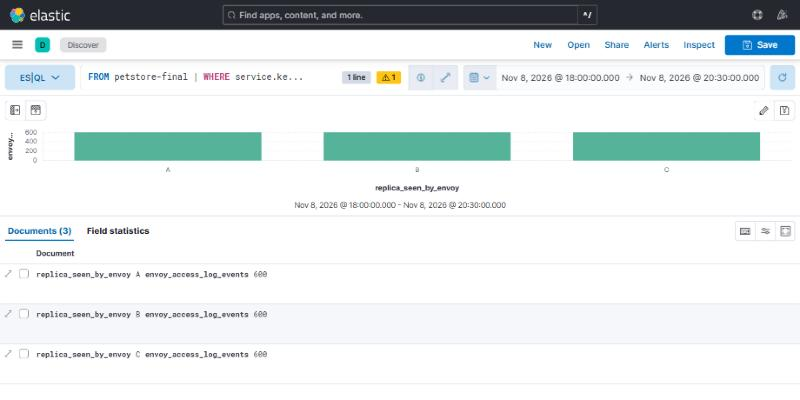
\includegraphics[width=0.85\textwidth]{figures/kibana-split.jpg}
\caption{Kibana (ES|QL): Envoy access-log events for the round-robin HTTP run, counted per replica. The query is
\code{FROM petstore-final | WHERE service.keyword == "envoy" AND request\_id.keyword LIKE "rr-equal-http-ecd47c-*" |
STATS COUNT(*) BY replica}.}
\label{fig:split}
\end{figure}

\section{Conclusions}

\begin{enumerate}[leftmargin=1.5em]
\item \textbf{Which strategy would I choose?}
  \begin{itemize}
  \item \textbf{HTTP: least request with active health checks.} When all replicas were healthy, it spread the load as
  evenly as round robin. When B was slow, it sent about 40\,\% fewer requests to B, while round robin kept sending it
  a full third. Health checks limited a crash to 1.3--1.8\,\% errors.
  \item \textbf{gRPC: the same, but Envoy must use HTTP/2 for gRPC.} Through a plain TCP proxy, 100\,\% of the calls
  went to one replica, because a gRPC client uses one connection. With HTTP/2 the calls were spread evenly.
  \end{itemize}
\item \textbf{A workload where I would choose differently.} If the replicas had \emph{different, known capacity},
for example A on a machine twice as powerful as B and C, I would use \textbf{weighted round robin} with weights that
match capacity (such as 2:1:1). D.1 showed that Envoy follows weights very exactly, while least request only reacts
after requests start to queue.
\item \textbf{What happens if Envoy stops?} Envoy is a single point of failure. Every HTTP request and gRPC call would
fail, even though A, B and C are healthy. Prometheus would still show the replicas as up, because it scrapes them
directly. \textbf{Improvement} (not implemented): run two or more Envoy instances behind a shared virtual IP or a
cloud load balancer, so that one Envoy can fail without taking the shop down.
\end{enumerate}

\textbf{Limitations.} Everything ran on one laptop with Docker Desktop, and short Docker pauses sometimes delayed a
few client requests. Response-time percentiles come from histogram buckets, so they are approximate; the smallest
bucket is 5\,ms. Active requests are only sampled every 5\,s.

\textbf{Sources and reuse.} This work builds on my Assignment 1 (metrics, Grafana, ELK logging) and Assignment 2
(REST API, gRPC service, idempotency, rate limiting). I used the Envoy documentation on load-balancing policies (round
robin, weighted, least request) and on active health checking, and the gRPC Health Checking Protocol. The README of
the repository has every command needed to repeat the runs, and the raw results are in the folder \code{results/}.

\end{document}
